\documentclass[aspectratio=43]{beamer}
\usetheme{CCNU}
%\usefonttheme[onlymath]{serif}

\usepackage{slashed}
\usepackage{datetime}
%\usepackage{slidesphysics}
\graphicspath{{../img/}}
\usepackage{hyperref}
\usepackage{cancel}
% \hypersetup{colorlinks=true, 
%     linkcolor=blue,          % color of internal links (change box color with linkbordercolor)
%     citecolor=black,        % color of links to bibliography
%     filecolor=black,      % color of file links
%     urlcolor=blue    }
% \usepackage{deflamb}
% \usepackage{color, colortbl}
% \usepackage{tikz}
%\usepackage{userdef}
\usepackage[absolute,overlay]{textpos}
\def\Put(#1,#2)#3{\leavevmode\makebox(0,0){\put(#1,#2){#3}}}

\def\mydate{\leavevmode\hbox{\the\year-\twodigits\month-\twodigits\day}}
\def\twodigits#1{\ifnum#1<10 0\fi\the#1}

\newcommand\Wider[2][3em]{%
\makebox[\linewidth][c]{%
  \begin{minipage}{\dimexpr\textwidth+#1\relax}
  \raggedright
  \centering#2
  \end{minipage}%
  }%
}

%\def\meetingname{Alicia Garrido Peña. PhD thesis Presentation}


\def\meetingname{Alicia Garrido Peña. PhD thesis Seminar}

\title[\meetingname]{Characterization of the sequential nature of neuronal dynamics: Experimental recordings, computational models and novel stimulation neurotechnologies}
\author[A. Garrido-Peña]{Alicia Garrido Peña}
% \institute[Michigan]{}
\institute[UAM]{Universidad Autónoma de Madrid}
\date[\mydate]{\meetingname\\\today}

\begin{document}
\begin{frame}[plain,t]
\titlepage
\end{frame}

%The next statement creates the title page.
\begin{frame}
\frametitle{Contents}
\tableofcontents
\end{frame}
%------------------------------------------------------------
\section{Introduction}
    \begin{frame}{Introduction}
	
	\subsection{Neuronal and networks dynamics}
	
	\subsection{The sequential nature of neural dynamics}
		\begin{minipage}[b]{0.5\textwidth}
			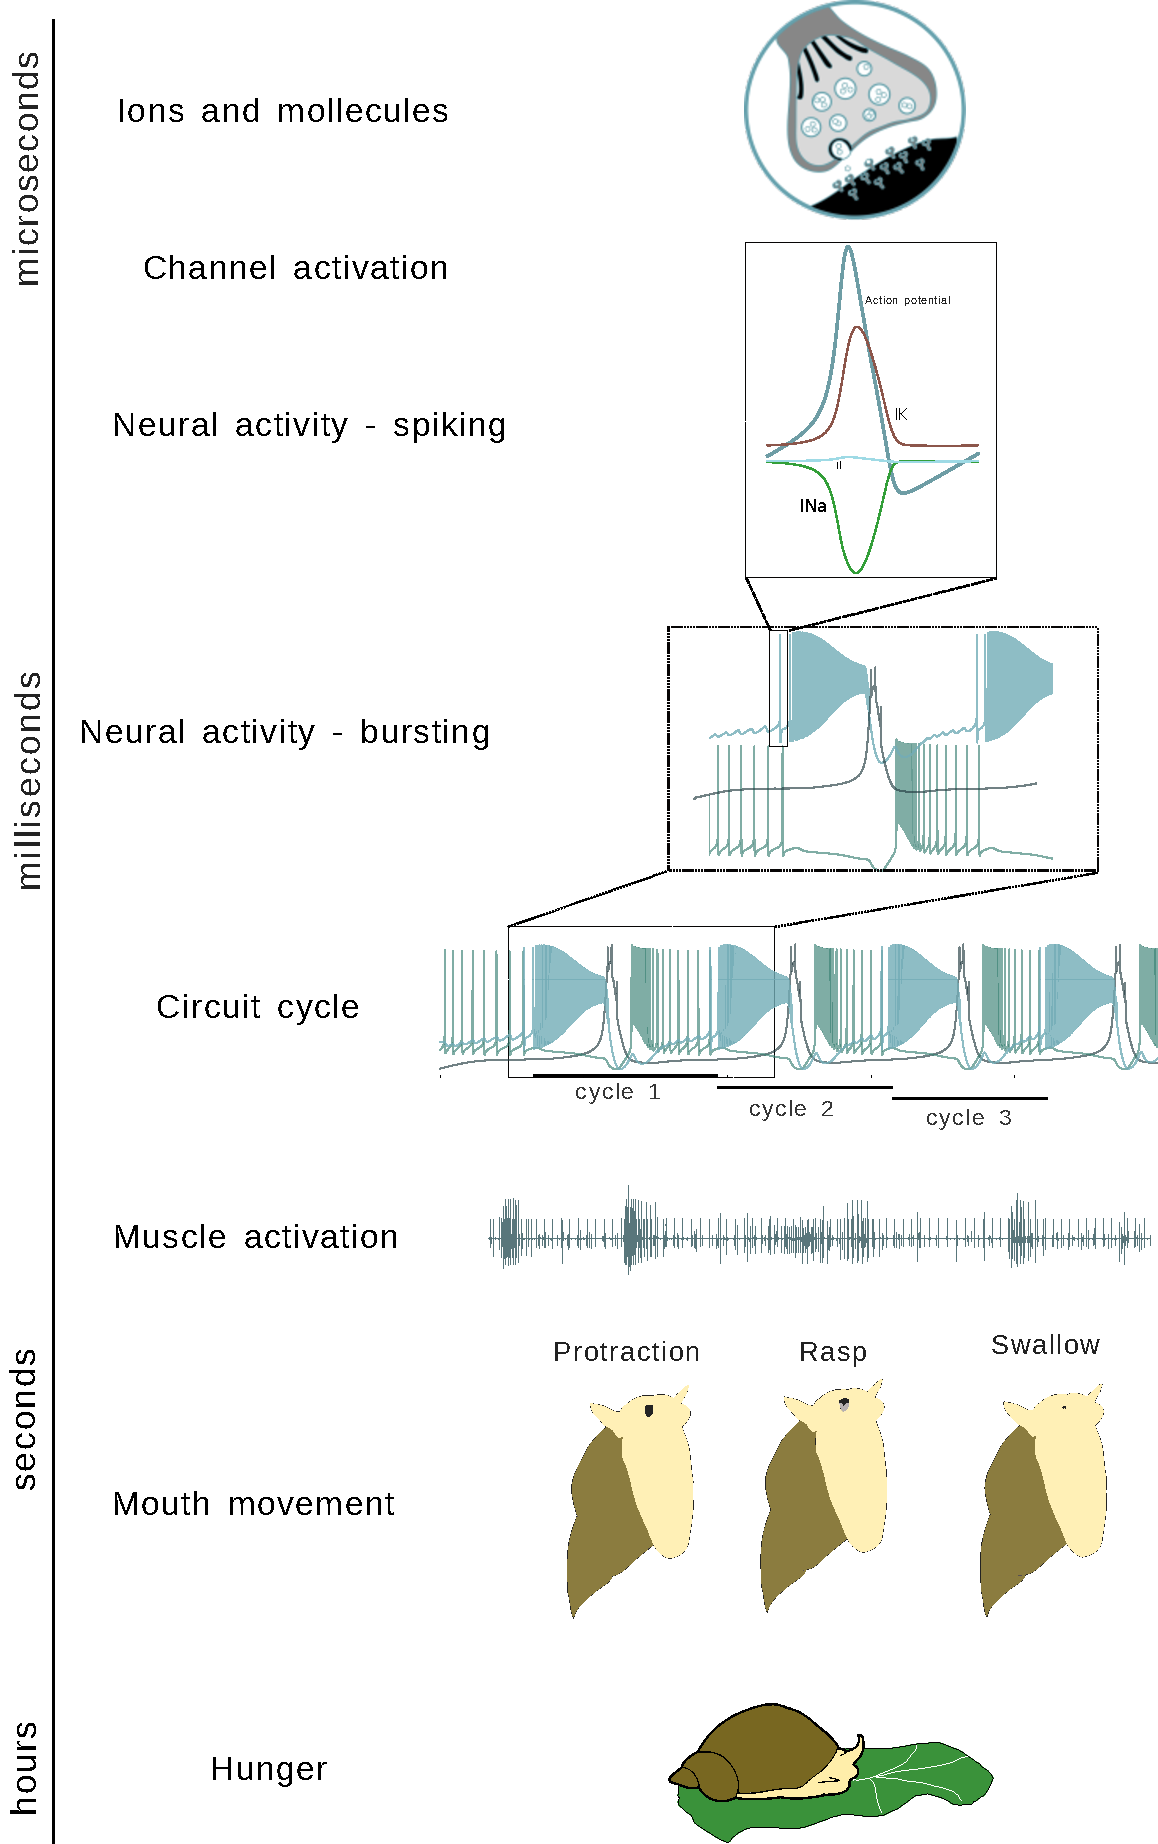
\includegraphics[width=\textwidth]{intro/time scale/time-scale-feeding.pdf}
		\end{minipage}
		\begin{minipage}[b]{0.4\textwidth}
		    \begin{itemize}
		    	\item There are sequential processes at different time-scales.
		    \end{itemize}
		\end{minipage}
    
    \subsection{Studying neural dynamics in computational models}
    \subsection{Vertebrate and invertebrate animal studies}
    \subsection{Neural stimulation}
    
	\end{frame}


\section{Motivation and Objectives}
\begin{frame}{Introduction}
	\subsection{Neuronal and networks dynamics}
	
	\subsection{The sequential nature of neural dynamics}
	\begin{minipage}[b]{0.5\textwidth}
		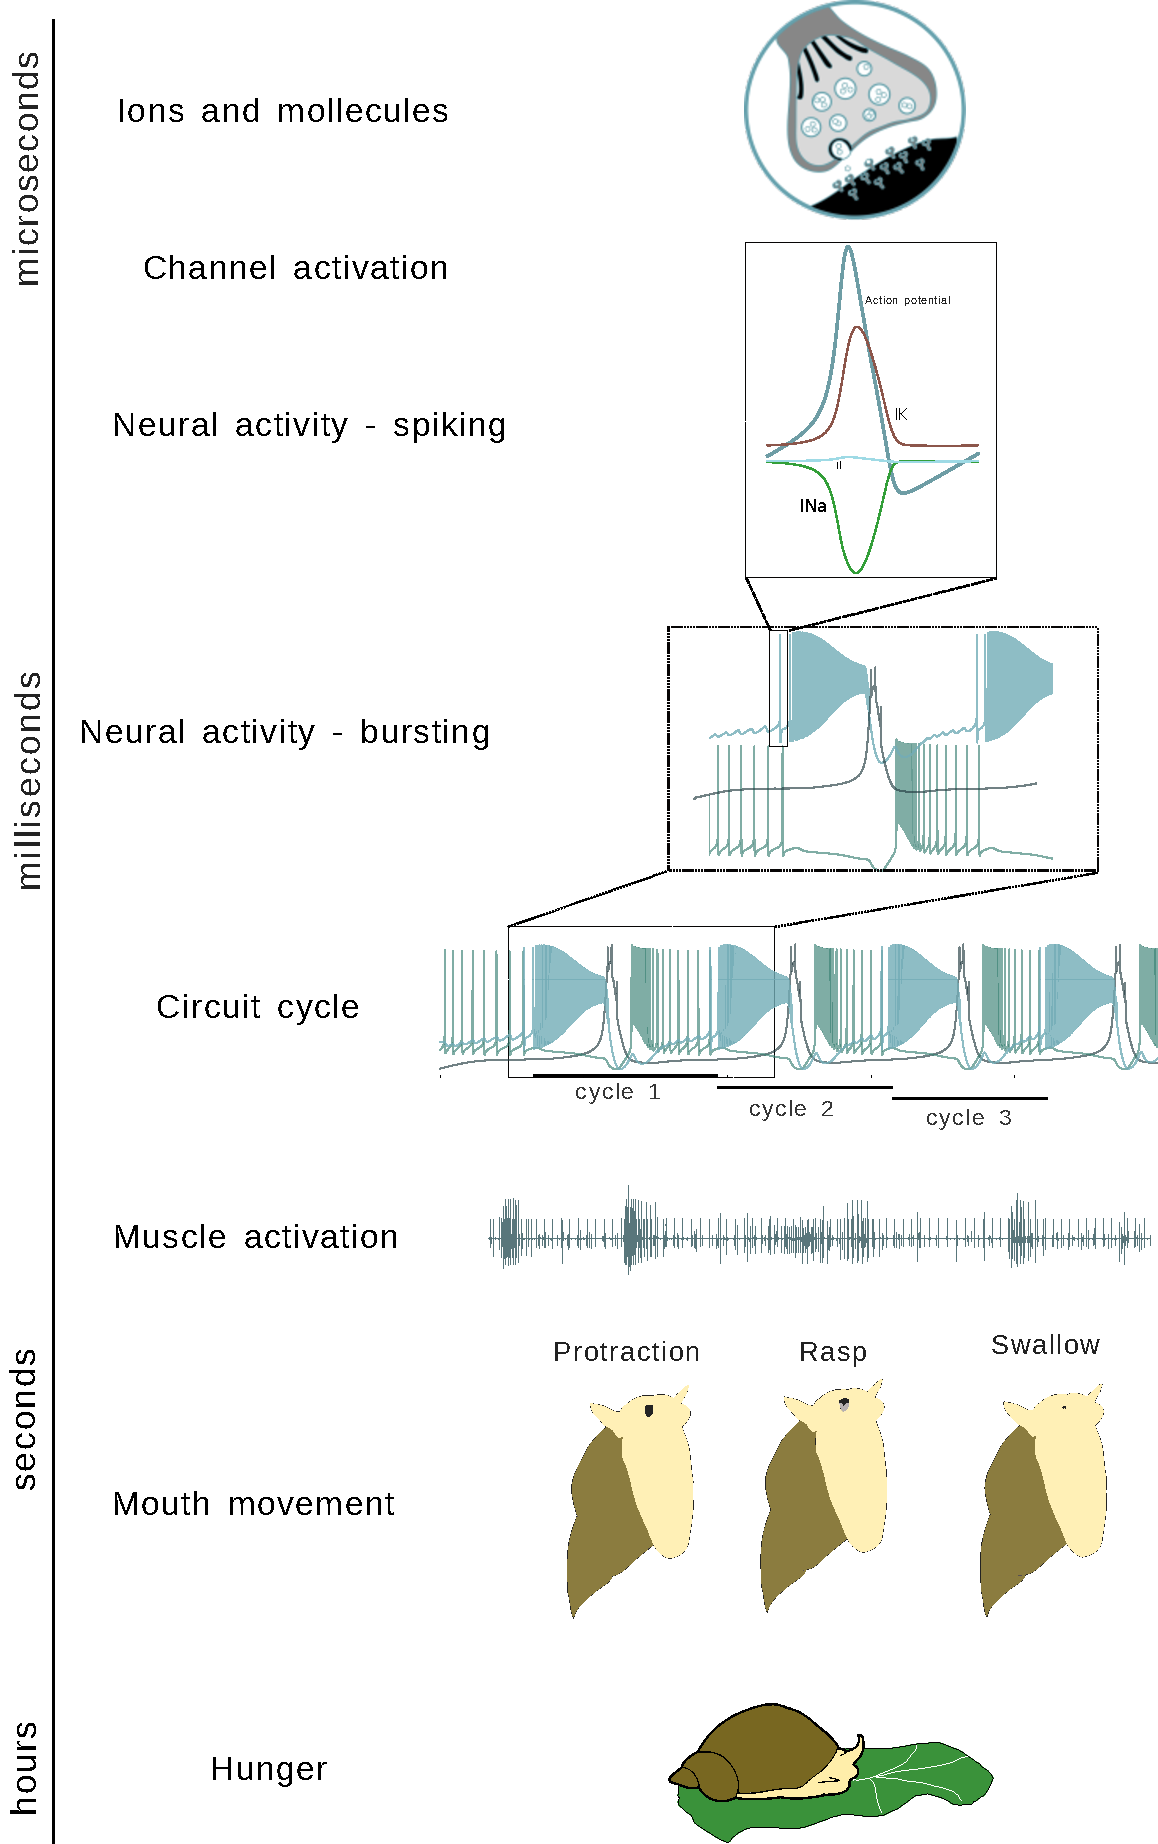
\includegraphics[width=\textwidth]{intro/time scale/time-scale-feeding.pdf}
	\end{minipage}
	\begin{minipage}[b]{0.4\textwidth}
		\begin{itemize}
			\item There are sequential processes at different time-scales.
		\end{itemize}
	\end{minipage}
	
	\subsection{Studying neural dynamics in computational models}
	\subsection{Vertebrate and invertebrate animal studies}
	\subsection{Neural stimulation}
\end{frame}


\section{Conclusion}

    \begin{frame}{Conclusion}
    
    \begin{itemize}
        \item $A+B=C$
        \item $p_T=13$
    \end{itemize}
    \end{frame}
%}
%\setbeamercolor{background canvas}{bg=violet}
\setbeamercolor{background canvas}{bg=CCNUMaize}
\begin{frame}[plain,t]
\vspace{100pt}
\centering

\includegraphics[width=0.6\textwidth]{logos/UAM+EPS_L-eps-converted-to.pdf}
\end{frame}
\end{document}